\documentclass[10pt]{article}
\usepackage[a4paper,margin=18mm]{geometry}
\usepackage{graphicx,hyperref,amsmath,booktabs}
\hypersetup{colorlinks=true,urlcolor=blue}
\setlength{\parindent}{0pt}\setlength{\parskip}{5pt}
\begin{document}
\begin{center}\Large Unknown indices inside the original six-member system\\[3pt]
\normalsize Curve25519 indexed circuit v1 --- unsigned producer evidence --- 16 November 2026\end{center}
The new Rust compiler appends unknown $t$ bits, exact finite-index range
guards, deterministic slack borrows and public constant-product gates.
All 1,059 original variables and 1,089 original equations remain literal
prefixes of the 1,989-variable, 2,223-equation augmented system (6,905 terms,
degree at most 2). Native PCC-20261116-b3227f. [pcc:unverified]

\textbf{Actual scope.} The parameters stay $p=2^{255}-19$, $A=486662$,
$a=60824497$, $q=213156431$, $k=20633$, with the original torus generator.
The SAME known original six-member witness extends and replays through
the original signed-index row and point sum. All 1,989 single-variable
mutations, wrong-target, malformed shape and the $t=q$ alias are refused.
Labels enter only the extension qualification helper. Zero solver invocations:
this stage does not discover a new root. [pcc:unverified]

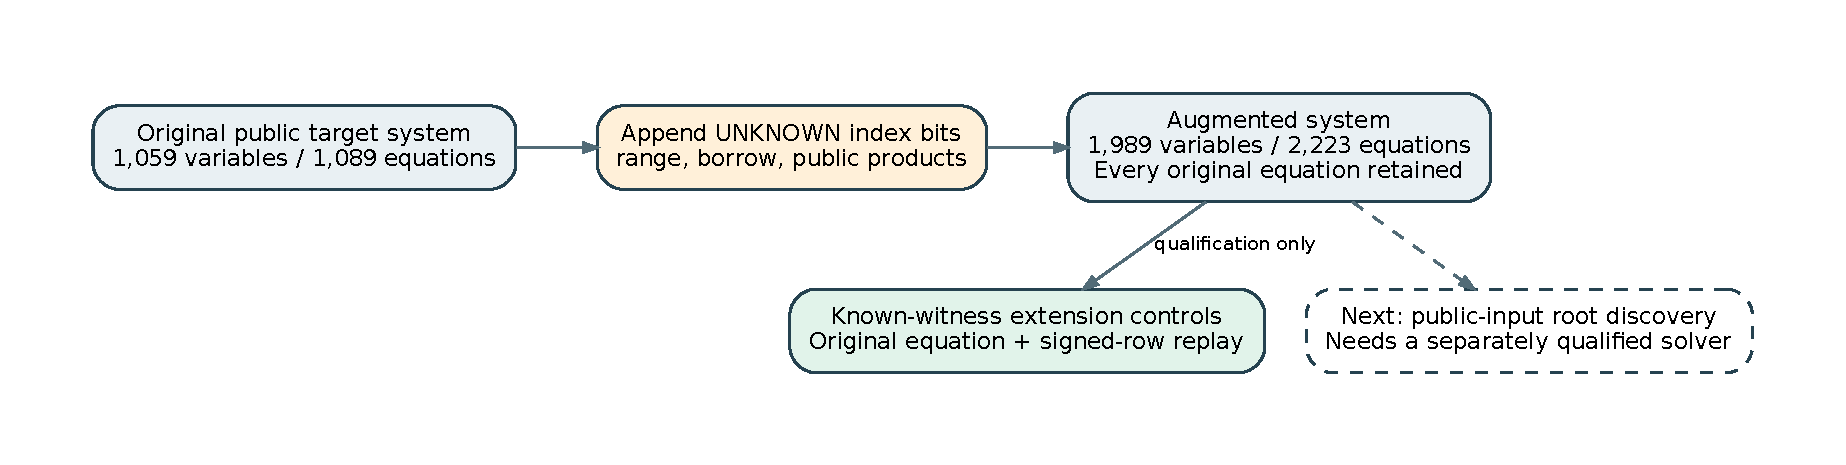
\includegraphics[width=\linewidth]{pipeline.pdf}

\textbf{Fixed native correspondence controls.}
The four complete Fp101 membership domains retain the following observations.
Index strings are exhausted on original roots; arbitrary auxiliary field
assignments are not exhaustively enumerated. [pcc:unverified]
\begin{center}\begin{tabular}{lrrr}\toprule
Fixture & Field pairs & Original roots & Canonical index checks\\\midrule
$a17,q3,k8$ &81,608&24&96\\
$a51,q2,k2$ &20,402&4&8\\
$a3,q17,k1$ &10,201&17&544\\
$a17,q1,k1$ &10,201&1&1\\\bottomrule
\end{tabular}\end{center}
All 24,024 original toy signed-pair/target decisions agree; 1,848 accepted
assignments replay original rows. Raw aliases stay distinct, and the original
two identity columns remain excluded. The 146,436-byte comparison trace is
retained as a 1,436-byte gzip. These are fixed development controls, not
useful-target yield. [pcc:unverified]

Of 279 toy overflow refusals, 23 labels already produce the SAME parameter:
coordinate equality alone cannot enforce a canonical index. Twelve malformed
constructor cases cover field chart, order, norm, bounds and arity. Runtime
checks exact generator order; prime-field validity remains external.
[pcc:unverified]

\newpage
\begin{center}\Large Algebraic bridge, source identity and next gate\end{center}
\textbf{Conditional index argument.}
In a field, assume $h$ primitive of order $M=aq$; $g=h^a$ is primitive
of order $q$. From $z^q=(h^j)^q$ and $h\ne0$, put $r=z/h^j$:
$r^q=1$. Existing primitive-root laws give a unique $0\le t<q$ with
$g^t=r$, hence $h^j g^t=z$. This argument does not need prime $q$.

Lean PCC-20261116-77b508 instantiates those existing Mathlib laws at actual
$a,q$. The focused maintained gate audits three named theorems, zero failing
and zero trusted-native exceptions, with standard foundations. Endpoints:
\texttt{actual\_subgroup\_primitive}, \texttt{actual\_coset\_index\_exists},
\texttt{actual\_coset\_index\_unique}. Signed standing remains unverified.
[pcc:unverified]

\textbf{Missing formal bridge.}
The endpoints assume Field, nonzero $h$ and primitive-root contracts. They
do not certify native arithmetic, actual primality or the order checker,
Boolean/range/borrow/product compiler semantics, the full native root
bijection or curve/group replay. Public role metadata is bound to the pinned
original layout, not an arbitrary future compiler. The proof map retains
these gaps.

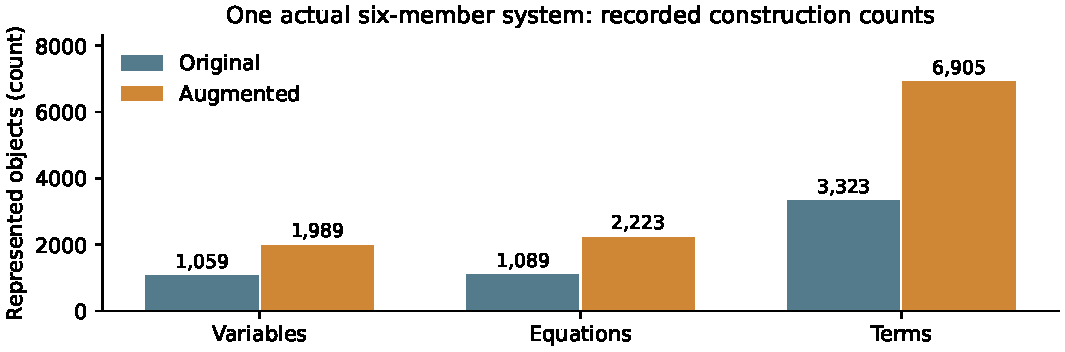
\includegraphics[width=\linewidth]{objects.pdf}
\textit{Counts of represented objects for one system; no solver-work,
time or memory comparison.} The construction adds 168 unknown index bits
and 762 deterministic variables. Extra constraints are not by themselves
evidence of cheaper discovery. [pcc:unverified]

\textbf{Reproducibility.}
The 49-input context reuses the unchanged 43-input, 55,368-byte v2 source
archive plus a 34,384-byte six-input delta. All source/archive/compiled hashes
match. A separately copied immutable qualifier and Rust pre-call commit
source/binary identities before controls. The retained binary SHA256 is
listed in \texttt{indexed-circuit-v1/FROZEN.md} and the source qualifier.
Release test/fmt/strict Clippy pass locally. The first redundant Lean tactic
and maintained audit advisories remain in raw evidence. [pcc:unverified]

\textbf{Next gate.}
Complete accounting and dependency propagation on identical public
original/augmented systems, charging failed branches and final original
replay. A separately admitted solver comparison must decide whether this
representation helps discovery. No paid job, timing, sampling campaign,
full-base enumeration or broad root-library rerun occurred.

\textbf{Sources and files.}
\href{https://cacr.uwaterloo.ca/hac/about/chap2.pdf}{HAC chapter2},
Facts2.170/2.172/2.173/2.213;
\href{https://cacr.uwaterloo.ca/hac/about/chap14.pdf}{chapter14},
Algorithms14.9/14.76/14.79; pinned Mathlib primitive-root source and existing
source review PCC-20261116-3aeb9e. KB unavailable; direct primary sources read.
Classical constructions are not claimed novel.
See \texttt{indexed-circuit-v1/} protocol/qualifier/native records and
\texttt{lean-indexed-v1/PROOF\_MAP.md}. Canonical performance graphs are
unchanged: this component adds no admitted performance datum.
\end{document}
